\documentclass{classrep}
\usepackage[utf8]{inputenc}
\frenchspacing

\usepackage{graphicx}
\usepackage[usenames,dvipsnames]{color}
\usepackage[hidelinks]{hyperref}
\usepackage{lmodern}
\usepackage{placeins}
\usepackage{url}
\usepackage{amsmath, amssymb, mathtools}
\usepackage{listings}
\usepackage{fancyhdr, lastpage}

\pagestyle{fancyplain}
\fancyhf{}
\renewcommand{\headrulewidth}{0pt}
\cfoot{\thepage\ / \pageref*{LastPage}}

%--------------------------------------------------------------------------------------%
\studycycle{Informatyka stosowana, studia dzienne, II st.}
\coursesemester{II}

\coursename{Analiza danych złożonych}
\courseyear{2021/2022}

\courseteacher{dr hab inż. Agnieszka Duraj}
\coursegroup{Czwartek, 14:00}

\author{%
    \studentinfo[239671@edu.p.lodz.pl]{Jan Karwowski}{239671}\\
    \studentinfo[239676@edu.p.lodz.pl]{Kamil Kowalewski}{239676}\\
}

\title{Referat wykładowy: Segmentacja semantyczna za pomocą sieci neuronowych}

\begin{document}
    \maketitle
    \thispagestyle{fancyplain}

    \tableofcontents
    \newpage


    \section{Wprowadzenie do segmentacji semantycznej} {

        % segmentacja semantyczna
        Segmentacja semantyczna (ang. \emph{semantic segmentation}) jest związana z danymi obrazowymi i
        polega na klasyfikacji każdego pixela z osobna do jednej z predefiniowanych klas. Oznacza to
        wyodrębnienie fragmentów obrazu stanowiących logiczną całość - najczęściej fragmentów
        reprezentujących pewne rzeczywiste obiekty. Wynikiem segmentacji semantycznej jest więc maska lub
        zbiór masek, w zależności od liczby rozpoznawanych klas obiektów. Na rysunku
        \ref{fig:semantic_segmentation_example} przedstawiona została przykładowa segmentacja semnatyczna
        obrazu ulicy. Różne kolory odpowiadają różnym klasom obiektów.

        \begin{figure}[!htbp]
            \centering
            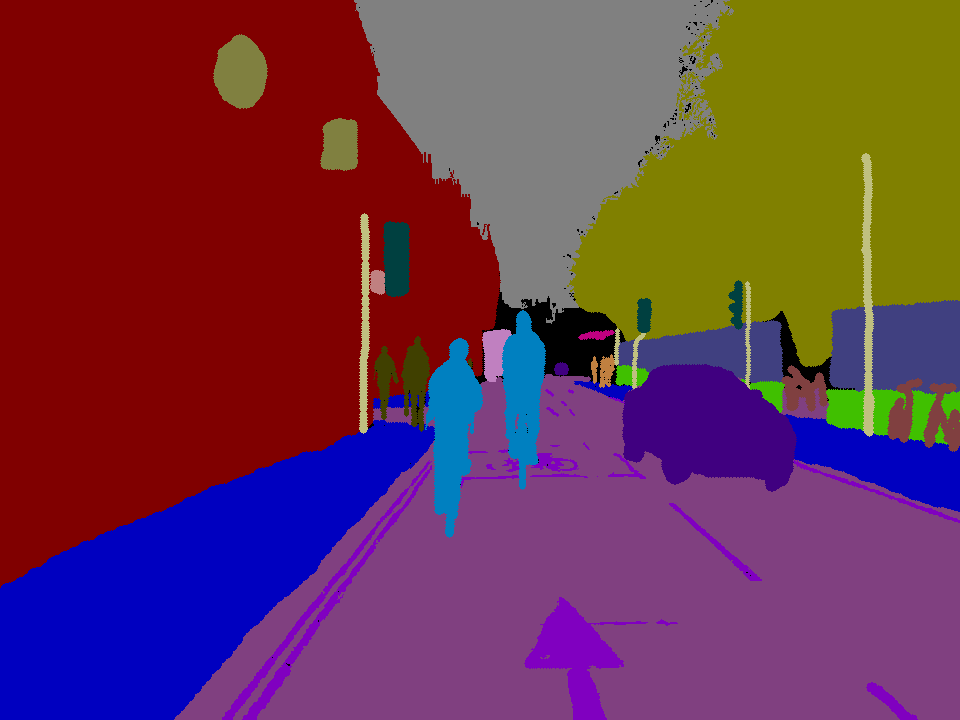
\includegraphics[width=\textwidth]{img/semantic_segmentation_example.png}
            \caption{Przykładowa segmentacja semantyczna \cite{url:semantic_segmentation_example}}
            \label{fig:semantic_segmentation_example}
        \end{figure}
        \FloatBarrier

        % segmentacje medyczne
        Segmentacja semantyczna nie jest ograniczona ani do obrazów prezentujących ludzi, drzewa czy
        samochody, ani w ogóle do kolorowych obrazów dwuwymiarowych. Okazuje się ona być szczególnie
        przydatna w przypadku obrazów medycznych. I tak np. segmentacja zmian chorobowych w mózgu czy w
        płucach, jak również segmentacja struktur anatomicznych danej części ciała, może bardzo pomóc w
        diagnozowaniu i leczeniu chorób. Jak wspomniano, segmentowane obrazy mogą być zarówno dwu jak i
        trójwymiarowe, przykład segmentacji wyników rezonansu magnetycznego mózgu (obraz 3D) przedstawiono
        na rysunku \ref{fig:medical_semantic_segmentation_example}.

        \begin{figure}[!htbp]
            \centering
            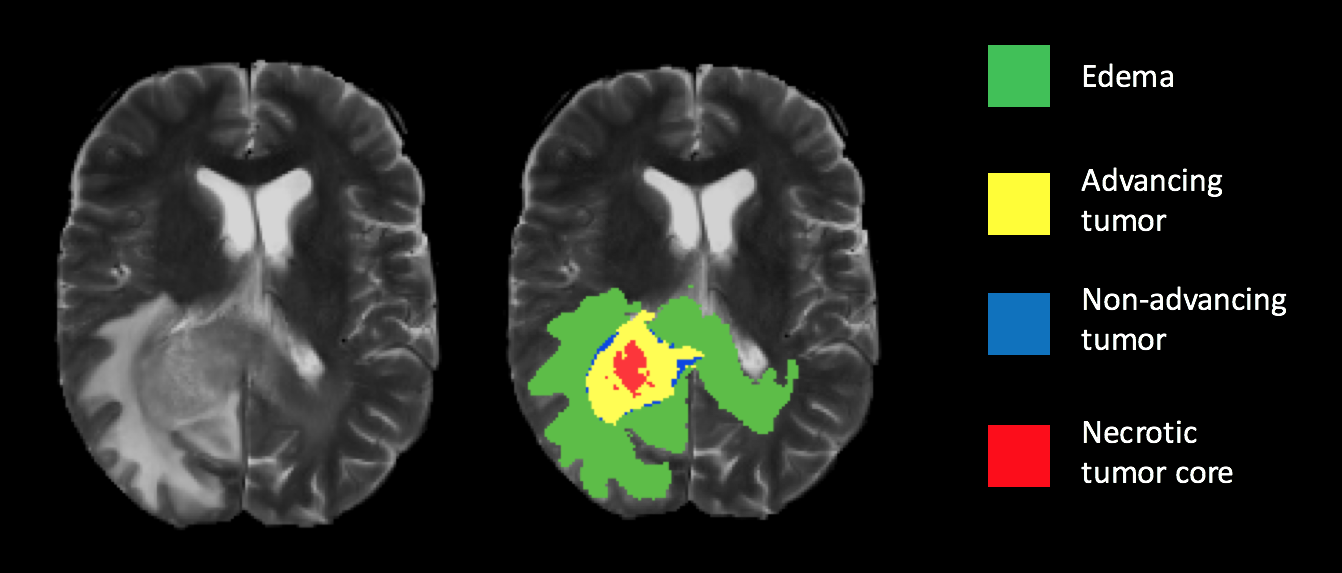
\includegraphics[width=\textwidth]{img/medical_semantic_segmentation_example.png}
            \caption{Przykładowa segmentacja guzów w mózgu \cite{url:medical_semantic_segmentation_example}}
            \label{fig:medical_semantic_segmentation_example}
        \end{figure}
        \FloatBarrier

        % rozpoznawanie obiektów i instance segmentation
        Z użytkowego punktu widzenia segmentacja semantyczna jest więc bardziej szczegółowym podejściem do
        rozpoznawania obiektów (ang. \emph{object detection}), które z kolei polega na zaznaczeniu obiektu
        na obrazie za pomocą prostokątnej ramki (ang. \emph{bounding box}). Zadania te, mimo iż ich wynik
        jest zupełnie różny, są dosyć mocno powiązane, co widać podczas porównania architektur sieci
        neuronowych realizujących zarówno to pierwsze jak i drugie zadanie. Istnieją również takie modele,
        które realizują oba te zadania jednocześnie - mamy wtedy do czynienia z tzw. \emph{instance
        segmentation}. Oznacza to, że nie tylko przeprowadzona jest segmentacja semantyczna obrazu, ale
        dodatkowo rozróżnione są poszczególne egzemplarze klas tego samego typu (np. różne samochody lub
        ludzie), co nie ma miejsca w przypadku zwykłej segmentacji semantycznej. Właściwie sprowadza się to
        do przeprowadzania kolejno klasycznego rozpoznawania obiektów, a nastepnie segmentacji semantycznej
        z pojedynczą klasą dla każdego z wyznaczonych wcześniej fragmentów obrazu zawierających jakieś
        obiekty. Przykładowy wynik realizacji zadania tego typu, jest przedstawiony na rysunku
        \ref{fig:instance_segmentation_example}.

        \begin{figure}[!htbp]
            \centering
            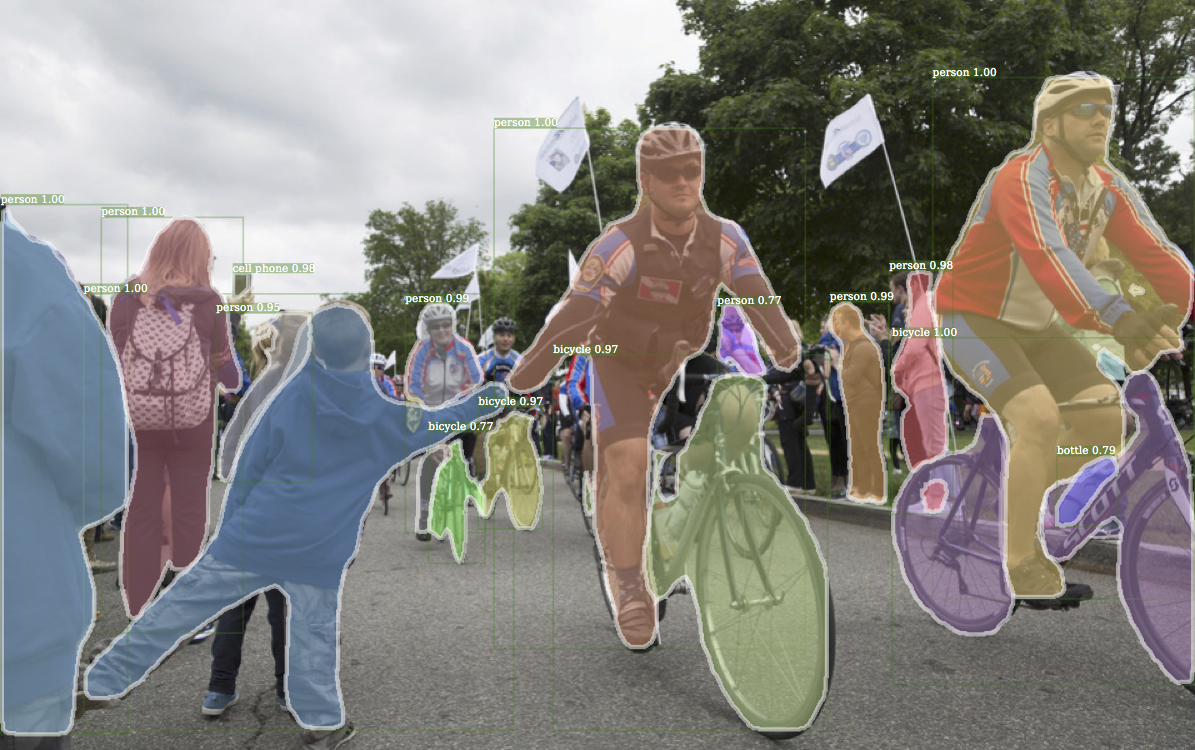
\includegraphics[width=\textwidth]{img/instance_segmentation_example.jpg}
            \caption
            {Przykładowy wynik rozpoznawania obiektów wraz z ich segmentacją semantyczną \cite{url:instance_segmentation_example}}
            \label{fig:instance_segmentation_example}
        \end{figure}
        \FloatBarrier

        % metryki
        W tym miejscu, podczas wprowadzania w temat segmentacji semantycznej, można jeszcze wspomnieć o
        sposobie oceniania jakości segmentacji. Tak jak w przypadku zadania klasyfikacji mamy do czynienia z
        bardzo popularnymi miarami jakości jak dokładność (\emph{accuracy}), czułość (\emph{recall}) czy
        precyzja (\emph{precision}), tak w przypadku segmentacji semantycznaj najczęściej wykorzystywane są
        \emph{IoU} (Intersection over Union) oraz \emph{Dice coefficient}. Pierwsza z nich jest równoznacza
        indeksowi Jaccarda, oblicza się ją dla danej klasy i zgodnie ze swoją nazwą oznacza wynik dzielenia
        sumy pikseli, gdzie segmentacja obliczona i oczekiwana się pokrywają, przez całkowitą liczbę pikseli
        jednej i drugiej segmentacji. Obrazuje to rysunek \ref{fig:iou}. Druga miara jest bardzo podobna i
        została zaprezentowana na rysunku \ref{fig:dice}. Można w różny sposób obliczyć wartości tych miar
        dla wielu klas, najprostszym podejściem jest wykorzystanie średniej arytmetycznej.

        \begin{figure}[!htbp]
            \centering
            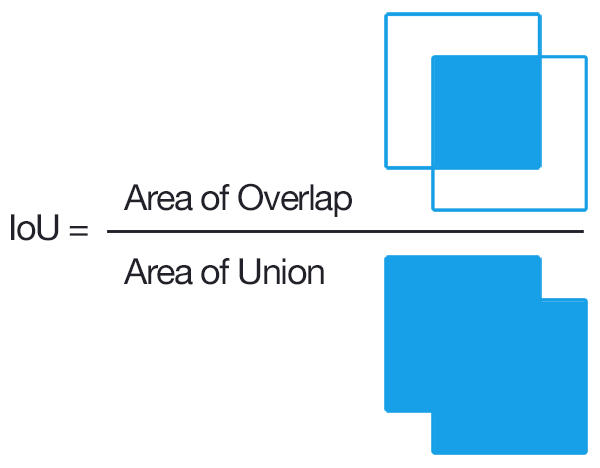
\includegraphics[width=0.6\textwidth]{img/iou.png}
            \caption{Miara jakości IoU \cite{url:iou}}
            \label{fig:iou}
        \end{figure}


        \begin{figure}
            \centering
            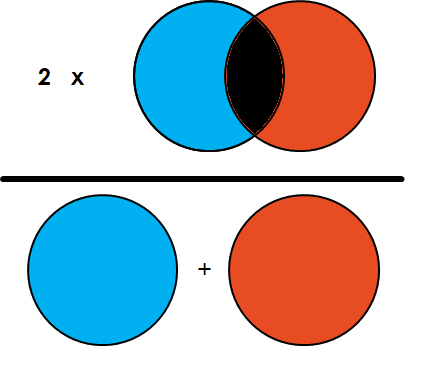
\includegraphics[width=0.6\textwidth]{img/dice.png}
            \caption{Miara jakości Dice coefficient \cite{url:dice}}
            \label{fig:dice}
        \end{figure}
        \FloatBarrier
    }

    \section{Problem ograniczonych zbiorów danych} {

        % problem zbiorów danych
        Zadanie segmentacji semantycznej można rozwiązać na wiele różnych sposobów. W ostatnich latach, wraz
        ze wzrostem popularności głębokich sieci neuronowych, to właśnie metody uczenia maszynowego okazują
        się najbardziej skuteczne w tej dziedzinie. Metody te wymagają jednak przygotowania dużych zbiorów
        danych, zawierających zazwyczaj zarówno przykładowe obrazy przeznaczone do segmentacji, jak i
        oczekiwane segmentacje. Wymóg przygotowania oczekiwanych segmentacji wynika z faktu, że w większości
        uczenie sieci neuronowych przebiega w sposób nadzorowany ("z nauczycielem"). Jest to o tyle
        problematyczne, że przygotowanie segmentacji semantycznej obrazu przez człowieka jest bardzo
        czasochłonne. W przypadku dwywmiarowego obrazu ulicy wystarczy kilkadziesiąt sekund do kilku minut i
        może zrobić to praktycznie każdy. Należy zwrócić uwagę, że to już i tak wielokrotnie więcej czasu
        niż w przypadku etykietowania obrazów przeznaczonych do klasyfikacji. W przypadku obrazów
        medycznych, gdzie granice segmentacji nie zawsze są jasne i wyraźnie widoczne, potrzebny jest
        specjalista (radiolog albo inny lekarz), który musi poświęcić temu zadaniu dużo uwagi. Dodając do
        tego fakt, że niektóre obrazy medyczne (np. wynik rezonansu magnetycznego czy tomografi
        komputerowej) są trójwymiarowe (składają się z wielu obrazów dwuwymiarówych, tzw. sliców), to
        przygotowanie segmentacji dla pojedynczego badania może zająć lekarzowi nawet do kilku godzin. Sieci
        neuronowe co do zasady wymagają do sprawnego funkcjonowania dużo danych uczących. Należy również
        pamiętać, że często jedynym sposobem poprawienia jakości działania modelu jest zebranie większej
        ilości danych. Okazuje się więc, że w przypadku zadania segmentacji semantycznej, zbiory danych
        stanowią szczególny problem. Istnieje oczywiście już bardzo wiele gotowych i ogólnodostępnych
        zbiorów danych, zarówno z obrazami medycznymi jak i np. z obrazami ulic, potrzebnymi do
        przygotowania modeli wykorzystywanych w branży automotive. Najbardziej popularnymi, ogólnodostępnymi
        zbiorami tego typu są m.in.: \emph{cityscapes} \cite{url:cityscapes}, \emph{COCO} \cite{url:coco},
        \emph{PASCAL VOC} \cite{url:pascal_voc} oraz dla danych medycznych np. \emph{BraTS} \cite{url:brats}.

        % metody unsupervised
        Coraz częściej stosowanym rozwiązaniem problemu ograniczonych danych uczących w zadaniu segmentacji
        semantycznej są metody uczenia nienadzorowanego. Podejście to zyskuje w ostatnim czasie bardzo dużą
        popularność i obecnie praktycznie wszystkie najlepsze osiągnięcia sieci neuronowych są oparte o
        jakąś formę uczenia nienadzorowanego. Dotyczy to nie tylko zadania segmentacji semantycznej ale w
        ogóle wszystkich zadań realizowanych przez sieci neuronowe, również, a może przede wszystkim, zadań
        z dziedziny przetwarzania języka naturalnego. Wynika to właśnie z ograniczonego dostępu do
        oznaczonych danych i bardzo szerokiego dostępu do nieoznaczonych danych (Internet). Uczenie
        nienadzorowane przybiera w tym przypadku właściwie dwie podstawowe formy. Pierwsza to
        \emph{Semi-Supervised Learning}, czyli uczenie ,,półnadzorowane''. Polega ono na wykorzystaniu
        bardzo małej ilości danych oznaczonych i dużej ilości danych nieoznaczonych. Najprostszym przykładem
        takiego algorytmu jest iteracyjne uczenie modelu najpierw na małej ilości danych oznaczonych przez
        człowieka, a następnie na pozostałych danych oznaczonych sztucznie za pomocą wyuczonego wcześniej
        modelu. Drugi rodzaj to \emph{Self-Supervised Learning}, czyli uczenie ,,samonadzorowane''. W tym
        przypadku korzysta się tylko z danych nieoznaczonych. Algorytmy te, podobnie zresztą jak algorytmu
        półnadzorowane, mogą być bardzo różne. Ogólnie jednak uczenie samonadzorowane polega na stworzeniu
        sztucznego zadania pomocniczego, które sieć rozwiązuje. Może to być np. układanie puzli czy
        wypełnianie luk w zdaniach. Tak wyuczony model może później zostać dotrenowany dla danego zadania na
        ograniczonym zbiorze danych (\emph{transfer learning}).

    }

    \section{Sieci neuronowe wykorzystywane do segmentacji semantycznej} {

        % wprowadzenie do sieci - przykładowy perceptron
        Jak wspomniano wcześniej, obecnie w celu realizacji zadania segmentacji semantycznej najczęściej
        wykorzystywane są sieci neuronowe. Te szczególne modele uczenia maszynowego mają już
        kilkudziesięcioletnią historię, która nie będzie tu omawiana. Dość wspomnieć, że obecnie technologia
        ta jest w fazie bardzo dynamicznego rozwoju, który zaczął się około roku 2012. Sieci neuronowe,
        składają się z warstw, które realizują funkcje wielowartościowe - każda warstwa to jedna funkcja.
        Sieć otrzymuje na wejście pewne dane (np. obraz) i zwraca pewien wynik - cała sieć jest właściwie
        bardzo złożoną funkcją matematyczną. Warstwy mają parametry, które są modyfikowane w trakcie
        treningu sieci tak, aby dla danego wejścia otrzymywać dane wyjście. Naprostszym przykładem sieci
        neuronowej jest \emph{perceptron wielowarstwowy}, gdzie warstwy realizują albo iloczyn skalarny
        parametrów (wag) z wartościami wejściowymi, albo tzw. funkcję aktywacji, którą może być np. funkcja
        sigmoidalna. Strukturę takiej sieci przedstawiono na rysunku \ref{fig:perceptron}.

        \begin{figure}[!htbp]
        \centering
        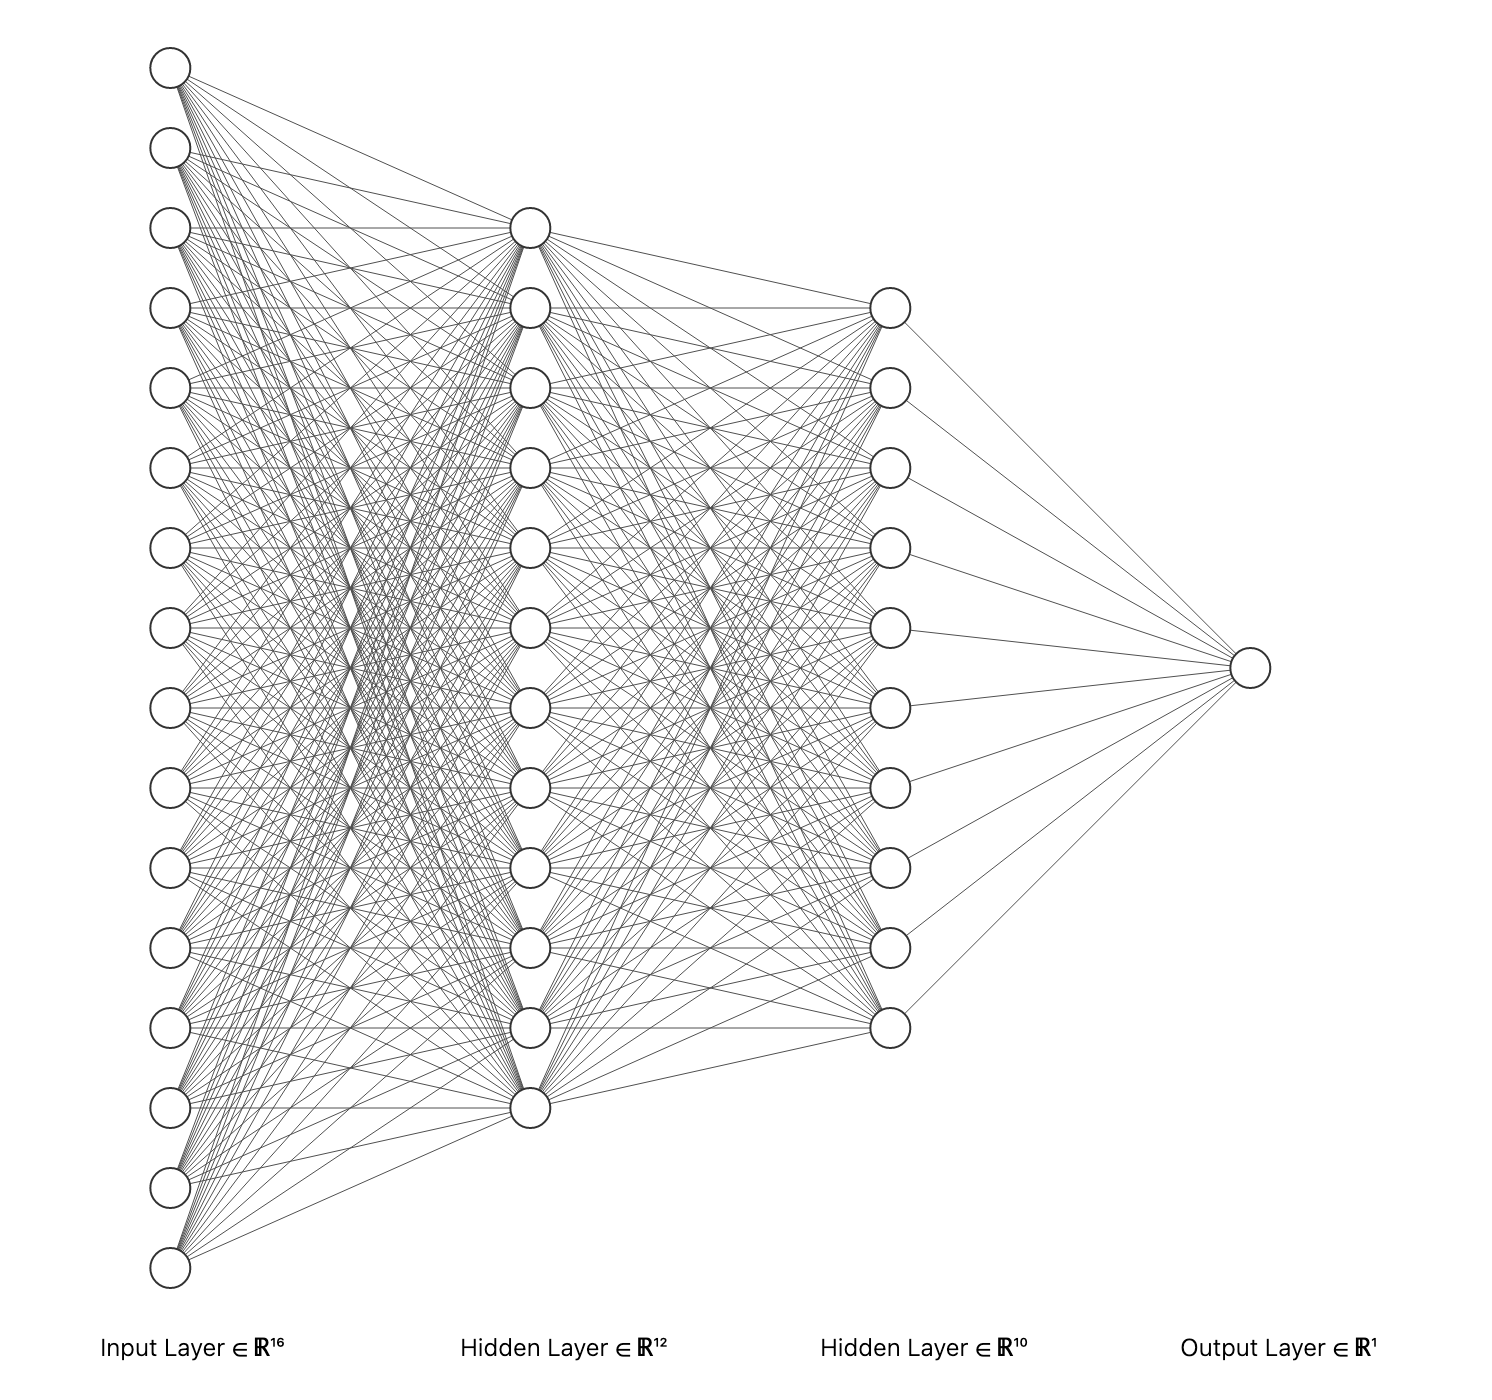
\includegraphics[width=0.7\textwidth]{img/perceptron.png}
        \caption{Struktura sieci perceptronu wielowarstwowego \cite{url:perceptron}.}
        \label{fig:perceptron}
        \end{figure}
        \FloatBarrier

        % różne rodzaje warstw
        Jak wspomniano, funkcje realizowane przez warstwy sieci neuronowej mogą być bardzo różne. W
        przypadku sieci przystosowanych do analizy obrazu, główną rolę grają tzw. warstwy splotowe. Warto
        wspomnieć, że w ostatnim roku wprowadzono do użycia w analizie obrazu inny rodzaj warstwy - tzw.
        self-attention, pochodządce z modeli sieci przeznaczonych do analizy języka naturalnego. Warstwy te
        sprawdziły się niezwykle dobrze i obecnie w najróżniejszy sposób są coraz chętniej wprowadzane do
        struktur sieci rozpoznających obrazy. Ogólnie rzecz ujmując, istnieje naprawdę bardzo wiele struktur
        sieci neuronowych służących do analizy obrazów. Z powodzeniem wykorzystuje się nawet wspomniany
        wcześniej perceptron wielowarstwowy, który użyty w odpowiedni sposób pozwala osiągnąć wyniki
        porównywalne z sieciami splotowymi i transformerami (modelami opartymi o warstwy self-attention).

        % automatyczna ekstrakcja cech
        Można powiedzieć, że co do idei, większość warstw każdej sieci neuronowej, niezależnie od ich
        rodzaju, realizuje zadanie \emph{automatycznej ekstrakcji cech} (ang. \emph{feature extraction}).
        Oznacza to, że kolejne funkcje (warstwy) transformują dane wejściowe do innej postaci. Jeżeli danymi
        wejściowymi jest pewien wielowymiarowy wektor (lub tensor), którego kolejne elementy mają przypisane
        pewne logiczne znaczenie, to na wyjściu każdej warstwy również znajdzie się wektor, w którymi
        elementy pełnią już zupełnie inną rolę. W ten sposób, wraz z przechodzeniem danych wejściowych przez
        kolejne warstwy, dane te są ,,kodowane'' w inny sposób, najczęściej tak, że ich znaczenie jest coraz
        bardziej abstrakcyjne. Przykład tego procesu został zaprezentowany na rysunku
        \ref{fig:feature_extraction}. Tak rozumiany ,,ekstraktor cech'' jest niezbędnym elementem sieci
        neuronowej, niezależnie od realizowanego zadania. W przypadku zadania klasyfikacji, wystarczy dodać
        na końcu sieci jedną warstwą, odpowiedzialną za klasyfikację. Będzie ona przyjmowała pewną
        wysokopoziomową reprezentację danych wejściowych i przyporządkowywała ją do odpowiedniej klasy. W
        procesie treningu takiej sieci, wagi dostosują się w ten sposób, aby ekstrahowane cechy miały
        znaczenie w kontekście realizowanego zadania. W przypadku innych zadań, część struktury sieci
        odpowiedzialna za realizację właściwego celu jest często bardziej złożona - taka sytuacja ma miejsce
        w przypadku segmentacji semantycznej.

        \begin{figure}[!htbp]
        \centering
        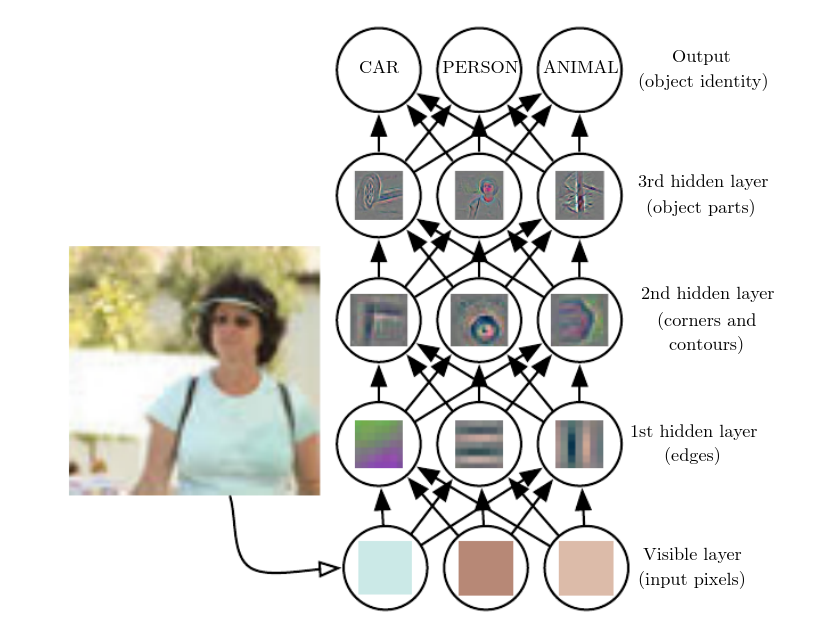
\includegraphics[width=\textwidth]{img/feature_extraction.png}
        \caption{Proces ekstrakcji cech w modelu sztucznej sieci neuronowej \cite{url:feature_extraction}.}
        \label{fig:feature_extraction}
        \end{figure}
        \FloatBarrier

        % u-net (warstwy splotowe)
        Przedstawiony zostanie teraz najbardziej podstawowy model sieci neuronowej stosowany powszechnie w
        zadaniu segmentacji semantycznej - \emph{U-Net}. Aby przedstawić strukturę tej sieci, niezbędne było
        wprowadzenie koncepcji automatycznej ekstrakcji cech. Sieć ta jest oparta o powszechnie stosowane w
        analizie obrazu warstwy splotowe. Warstwy te pełnią rolę filtrów, które są nakładane na obraz
        wejściowy, powodując powstanie tzw. map cech. Oznacza to, że dwuwymiarowy obraz po przejściu przez
        taką warstwę, pozostaje dwuwymiarą mapą występowania pewnego wzorca na oryginalnym obrazie. Dokładna
        zasada działania warstwy splotowej została przedstawiona na rysunku \ref{fig:conv}, a przykładowy
        wynik przetworzenia obrazu przez taką warstwę przedstawiono na rysunku \ref{fig:conv_example}.

        \begin{figure}[!htbp]
        \centering
        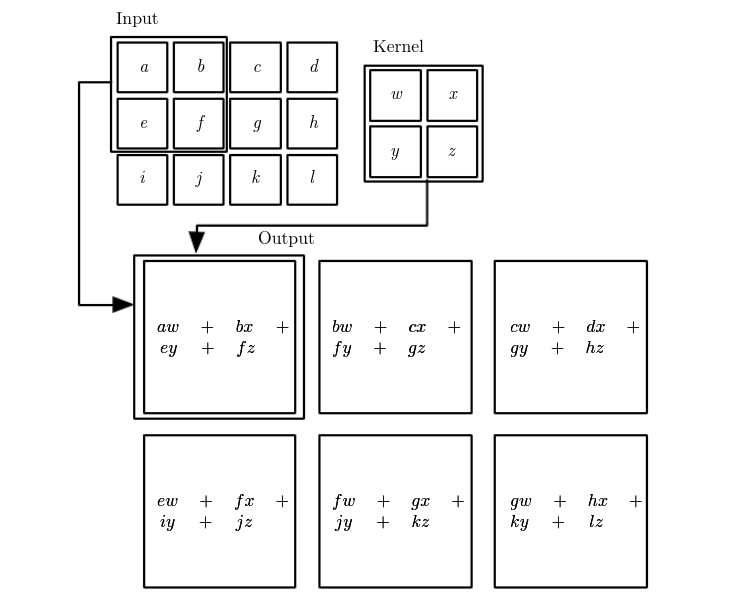
\includegraphics[width=\textwidth]{img/conv.png}
        \caption{Zasada działania warstwy splotowej \cite{url:conv}}
        \label{fig:conv}
        \end{figure}

        \begin{figure}[!htbp]
        \centering
        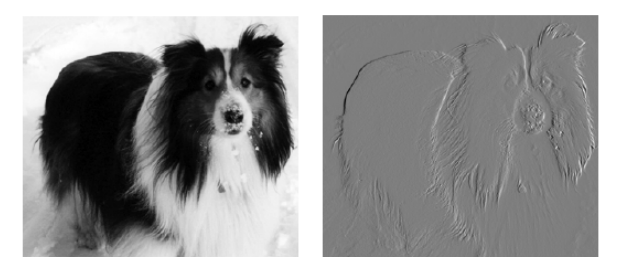
\includegraphics[width=\textwidth]{img/conv_example.png}
        \caption{Rozpoznawanie krawędzi poziomej jako przykład działania warstwy splotowej \cite{url:conv_example}}
        \label{fig:conv_example}
        \end{figure}
        \FloatBarrier

        % u-net architektura
        Struktura sieci U-Net została przedstawiona na rysunku \ref{fig:unet}. Składa się ona z dwóch
        części. Pierwszą z nich jest ekstraktor cech - lewe ramię sieci. Ekstraktor ten może mieć właściwie
        dowolną postać. Może to być odpowiednia część dowolnej sieci przystosowanej do klasyfikacji obrazów,
        jak chociażby \emph{ResNet} czy \emph{EfficientNet}. Takie ekstraktory cech, oparte o warstwy
        splotowe, charakteryzują się tym, że kolejne bloki (grupy warstw), zmniejszają rozmiar map cech. W
        konsekwencji wraz z przechodzeniem danych wejściowych przez kolejne warstwy, obraz ma coraz mniejsze
        wymiary przestrzenne i coraz więcej małych i bardziej abstrakcyjnych (wysokopoziomowych) co do
        znaczenia map cech. Dokładnie taka sytuacja ma miejsce również w przypadku zaproponowanego przez
        autorów oryginalnego U-Net'a ekstraktora cech (zwanego również powszechnie \emph{enkoderem}). Cały
        problem, którego rozwiązaniem jest zaproponowana architektura sztucznej sieci neuronowej, to jak
        wykorzystać te liczne i niewielkie mapy cech do wytworzenia segmentacji semantycznej obrazu.
        Najprostszym co można zrobić, to sztucznie powiększyć i połączyć te mapy cech (\emph{zresamplować}),
        tak aby odpowiadały rozmiarowy oryginalnego obrazka. Jak się okazuje takie rozwiązanie daje już
        całkiem ciekawe wyniki i jest czasami stosowane, kiedy kluczową rolę gra niewielki rozmiar sieci -
        jej szybkość i prostota. Jeżeli jednak chce się osiągnać nie tylko dobrą jakość klasyfikacji
        obiektów na obrazie (poprawne etykiety dla posczególnych pikseli), ale również ważne jest precyzyjne
        położenie obiektów, to potrzeba zastosować dodatkową technikę, jaką są w przypadku U-Net'u
        połączenia rezydualne z enkdora. Technika polega na tym, że coraz bardziej powiększane
        wysokopoziomowe mapy cech, są łączone z niskpoziomowymi ale większymi mapami cech, z wcześniejszych
        etapów ekstrakcji cech. W ten sposób uwzględniona zostaje informacja o dokładnym położeniu obiektów,
        która jest tracona, wraz z wyciąganiem bardziej abstrakcyjnych i silniejszych znaczeniowo cech
        obrazu.

        \begin{figure}[!htbp]
        \centering
        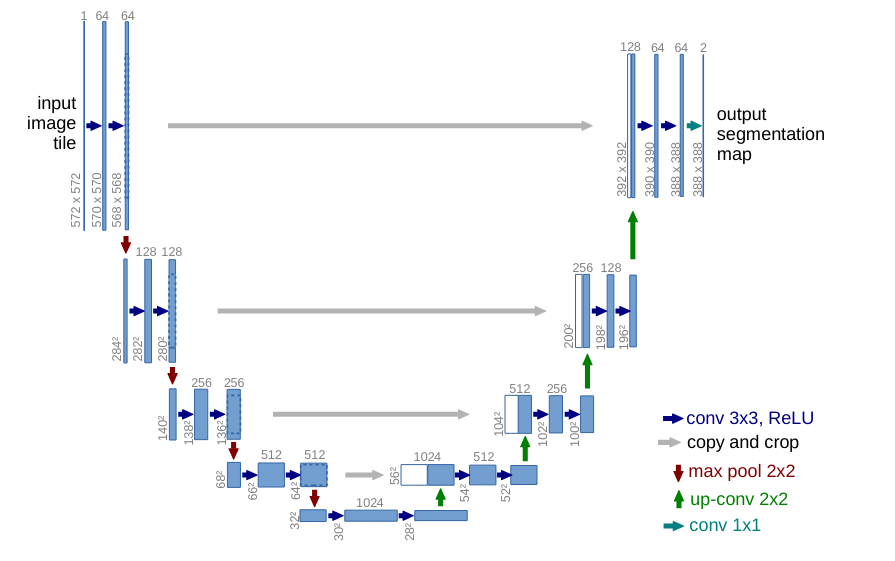
\includegraphics[width=\textwidth]{img/unet.png}
        \caption{Struktura sieciu U-Net \cite{url:unet}}
        \label{fig:unet}
        \end{figure}
        \FloatBarrier

        Przedstawiona architektura stanowi punkt wyjścia dla innych rozwiązań do przeprowadzania segmentacji
        semantycznej. W obecnej chwili jest to już mocno ugruntowany (rozwiązanie z 2015 roku) \emph{de
        facto} standard, zwłaszcza w dziedzienie segmentacji obrazów medycznych. Należy jednak pamiętać, że,
        jak wspomniano wcześniej, coraz to nowsze struktury i rodzaje warstw sieci neuronowych są
        wprowadzane do użytku i przedstawiony U-Net nie jest jedynym słusznym podejściem do segmentacji
        semantycznej. Istnieje zarówno bardzo wiele możliwych usprawnień tej metody, jak i zupełnie nowe
        podejścia.
    }

\begin{thebibliography}{0}
    \bibitem{book}{Ian Goodfellow et al (2016) \emph{Deep Learning}}
    \bibitem{paperswithcode}{https://paperswithcode.com/}
    \bibitem{url:semantic_segmentation_example}{http://mi.eng.cam.ac.uk/research/projects/VideoRec/CamVid/}
    \bibitem{url:medical_semantic_segmentation_example}{https://github.com/naldeborgh7575/brain\_segmentation}
    \bibitem{url:instance_segmentation_example}{https://github.com/facebookresearch/Detectron}
    \bibitem{url:iou}{https://en.wikipedia.org/wiki/Jaccard\_index}
    \bibitem{url:dice}{https://towardsdatascience.com/metrics-to-evaluate-your-semantic-\\segmentation-model-6bcb99639aa2}
    \bibitem{url:cityscapes}{https://www.cityscapes-dataset.com/dataset-overview/}
    \bibitem{url:coco}{https://cocodataset.org}
    \bibitem{url:pascal_voc}{http://host.robots.ox.ac.uk/pascal/VOC/}
    \bibitem{url:brats}{https://www.med.upenn.edu/sbia/brats2018/data.html}
    \bibitem{url:perceptron}{https://towardsdatascience.com/tagged/multilayer-perceptron}
    \bibitem{url:feature_extraction}{https://www.deeplearningbook.org/contents/intro.html}
    \bibitem{url:conv}{https://www.deeplearningbook.org/}
    \bibitem{url:conv_example}{https://www.deeplearningbook.org/}
    \bibitem{url:unet}{https://arxiv.org/abs/1505.04597}
\end{thebibliography}

\end{document}
